% Wrapped KDP paperback cover for On Hilbert's 6th Problem.
% Trim 7 x 10 in, black and white interior on white paper: spine = pages x 0.002252 in,
% full width = 0.125 + 7 + spine + 7 + 0.125 in, height 10.25 in. Build with the interior's page count,
%   pdflatex "\def\InteriorPages{$(pdfinfo ../main.pdf | awk '/^Pages/{print $2}')}% Wrapped KDP paperback cover for On Hilbert's 6th Problem.
% Trim 7 x 10 in, black and white interior on white paper: spine = pages x 0.002252 in,
% full width = 0.125 + 7 + spine + 7 + 0.125 in, height 10.25 in. Build with the interior's page count,
%   pdflatex "\def\InteriorPages{$(pdfinfo ../main.pdf | awk '/^Pages/{print $2}')}% Wrapped KDP paperback cover for On Hilbert's 6th Problem.
% Trim 7 x 10 in, black and white interior on white paper: spine = pages x 0.002252 in,
% full width = 0.125 + 7 + spine + 7 + 0.125 in, height 10.25 in. Build with the interior's page count,
%   pdflatex "\def\InteriorPages{$(pdfinfo ../main.pdf | awk '/^Pages/{print $2}')}% Wrapped KDP paperback cover for On Hilbert's 6th Problem.
% Trim 7 x 10 in, black and white interior on white paper: spine = pages x 0.002252 in,
% full width = 0.125 + 7 + spine + 7 + 0.125 in, height 10.25 in. Build with the interior's page count,
%   pdflatex "\def\InteriorPages{$(pdfinfo ../main.pdf | awk '/^Pages/{print $2}')}\input{cover}"   (twice),
% then check: kdp.py cover <interior.pdf> --cover cover.pdf. Without the definition the count below is used.
\providecommand\InteriorPages{548}
\documentclass{article}
\usepackage{tikz,graphicx,xcolor}
\pgfmathsetmacro\Spine{\InteriorPages*0.002252}
\pgfmathsetmacro\W{14.25+\Spine}
\pgfmathsetmacro\FrontL{7.125+\Spine}
\pgfmathsetmacro\FrontC{\FrontL+3.5}
\pgfmathsetmacro\SpineC{7.125+\Spine/2}
\usepackage[paperwidth=\W in,paperheight=10.25in,margin=0in]{geometry}
\usepackage[T1]{fontenc}
\usepackage[sc]{mathpazo}
\usepackage[none]{hyphenat}
\definecolor{navy}{HTML}{0F1B2D}
\definecolor{gold}{HTML}{D9B86C}
\definecolor{ivory}{HTML}{EFE6D2}
\pagestyle{empty}
\begin{document}
\noindent\begin{tikzpicture}[x=1in,y=1in,remember picture,overlay,shift={(current page.south west)}]
% background
\fill[navy] (0,0) rectangle (\W,10.25);
% front artwork, bleeding off right and bottom, cropped at the top below the authors
\begin{scope}
\clip (\FrontL,0) rectangle (\W,6.6);
\node[anchor=south west,inner sep=0] at (\FrontL,0) {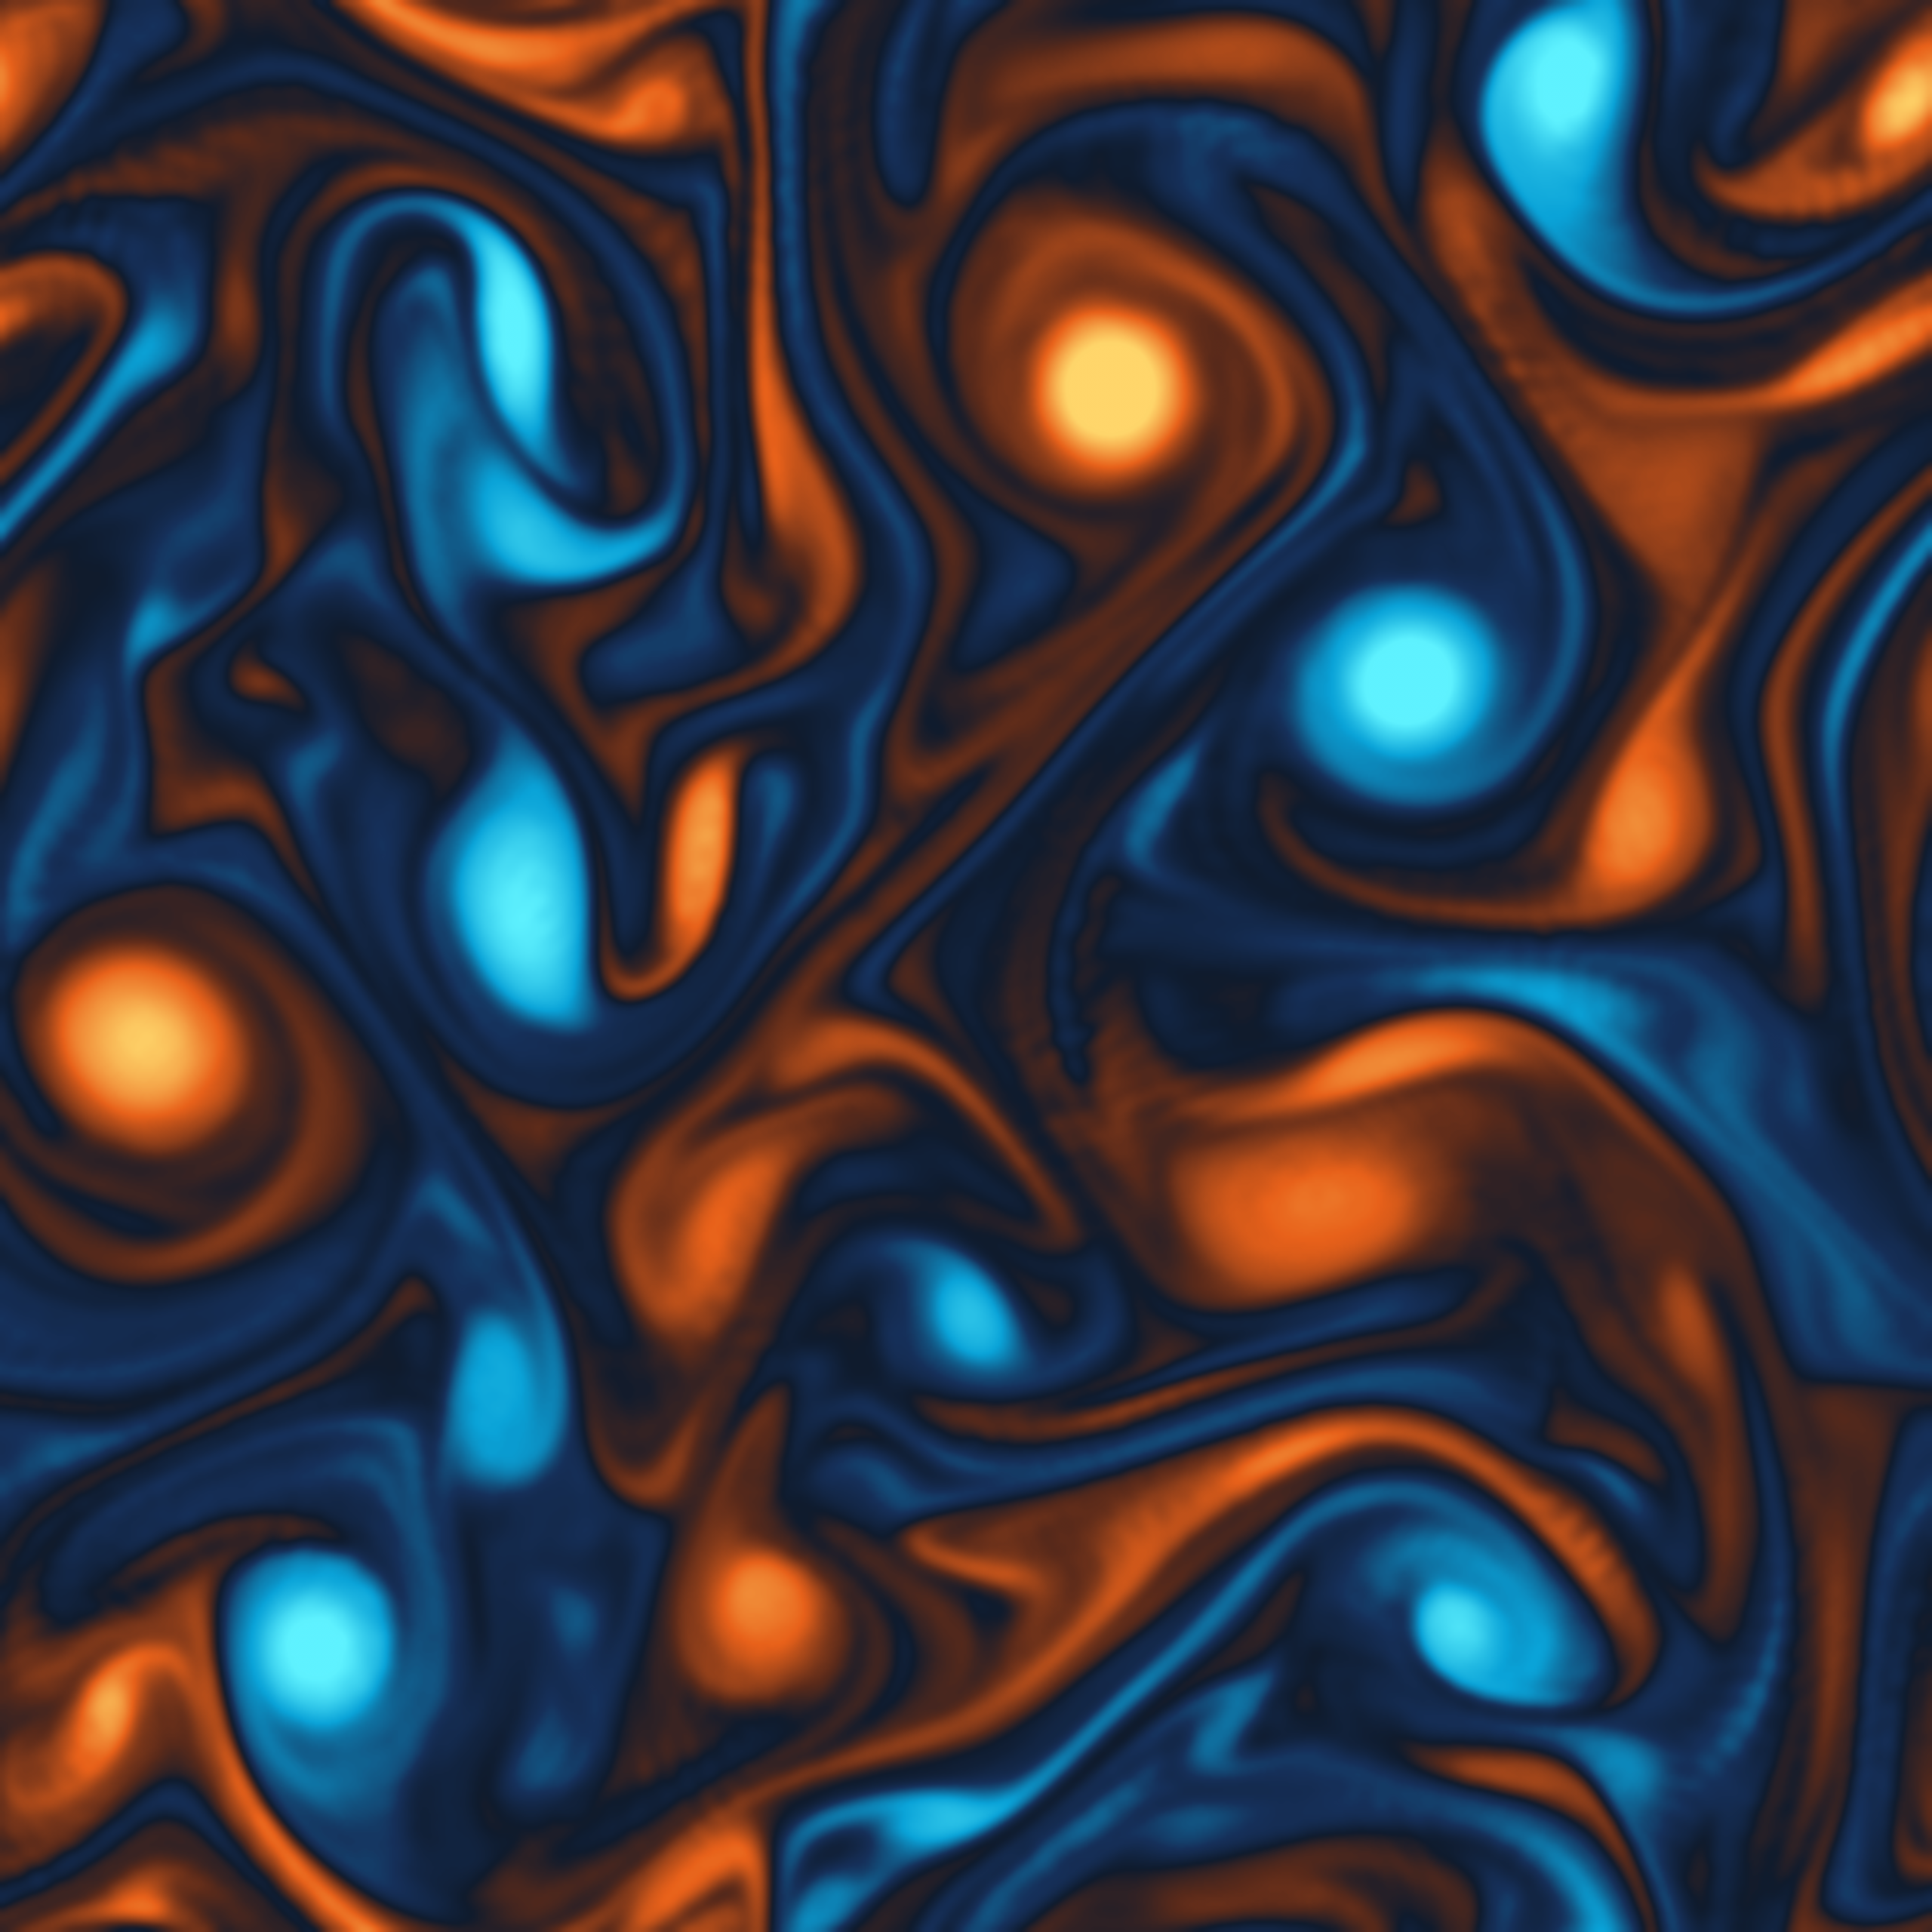
\includegraphics[width=7.125in]{art_ns.png}};
\end{scope}
% front text
\node[text=ivory,align=center] at (\FrontC,9.26) {\fontsize{42}{48}\selectfont\scshape On Hilbert's};
\node[text=ivory,align=center] at (\FrontC,8.49) {\fontsize{42}{48}\selectfont\scshape 6th Problem};
\draw[gold,line width=0.6pt] (\FrontC-1.33,7.90) -- (\FrontC+1.33,7.90);
\node[text=gold,align=center] at (\FrontC,7.45) {\fontsize{16.5}{21}\selectfont\itshape Probability, Mechanics and Bayesian Computation};
\node[text=ivory,align=center] at (\FrontC,6.93) {\fontsize{17.5}{22}\selectfont\scshape Nick Polson \quad\textperiodcentered\quad Vadim Sokolov};
% spine
\node[text=ivory,rotate=-90,anchor=center] at (\SpineC,6.21) {\fontsize{14}{16}\selectfont\scshape On Hilbert's 6th Problem};
\node[text=gold,rotate=-90,anchor=center] at (\SpineC,1.76) {\fontsize{11}{13}\selectfont\scshape Polson \,\textperiodcentered\, Sokolov};
% back cover blurb
\node[text=ivory,anchor=north west,text width=5.6in,align=justify] at (0.75,9.36) {%
\fontsize{11.25}{15.2}\selectfont
{\fontsize{16.5}{21}\selectfont\scshape\color{gold} From atoms to continua, and back\par}
\vspace{0.9em}
In 1900 David Hilbert asked for a mathematical treatment of the axioms of physics, beginning with probability and mechanics, and for the limiting processes that lead from the atomistic view to the laws of motion of continua. A century and a quarter later Kolmogorov's axioms have settled the first half, and the passage from hard spheres to the Boltzmann equation and on to the Navier Stokes equations has been carried out for long times.\par
\vspace{0.6em}
This book tells that story and adds a second half: the inverse passage, from observed fluids back to the states that produced them. Henri Poincar\'e, who examined Bachelier's thesis in the year of Hilbert's address, is a central figure, from recurrence and the method of arbitrary functions to the quanta and the conjecture that Perelman settled with an entropy from statistical mechanics.\par
\vspace{0.6em}
Topics include de Finetti and Sanov, Brownian motion and Yor's identities read as algorithms, Thorin measures and shot noise, Perelman's entropy and the uncertainty principle, Nelson's stochastic mechanics, Lanford's theorem and Kac's program, hydrodynamic limits, Bayesian inference on the Navier Stokes solution manifold with adjoint sufficient statistics and learned posterior generators, blowup and turbulence, Lee Yang zeros, Schr\"odinger bridges and generative Bayesian computation, filters and gates, and the thermodynamics of information. A final chapter builds a bridge to Hilbert's eighth problem through the de Bruijn Newman heat flow. A chapter on ergodic theory, a chapter on the method of types and moment conditioning, and a section on Lanford windows complete the foundations; every chapter closes with exercises, and computed figures illustrate the book throughout.\par
\vspace{0.9em}
{\itshape Nick Polson is Professor of Econometrics and Statistics at the Booth School of Business, University of Chicago. Vadim Sokolov is Associate Professor at George Mason University.}\par
};
% barcode area kept clear (KDP places barcode here)
\fill[white] (4.875,0.375) rectangle (6.875,1.575);
\end{tikzpicture}
\end{document}
"   (twice),
% then check: kdp.py cover <interior.pdf> --cover cover.pdf. Without the definition the count below is used.
\providecommand\InteriorPages{548}
\documentclass{article}
\usepackage{tikz,graphicx,xcolor}
\pgfmathsetmacro\Spine{\InteriorPages*0.002252}
\pgfmathsetmacro\W{14.25+\Spine}
\pgfmathsetmacro\FrontL{7.125+\Spine}
\pgfmathsetmacro\FrontC{\FrontL+3.5}
\pgfmathsetmacro\SpineC{7.125+\Spine/2}
\usepackage[paperwidth=\W in,paperheight=10.25in,margin=0in]{geometry}
\usepackage[T1]{fontenc}
\usepackage[sc]{mathpazo}
\usepackage[none]{hyphenat}
\definecolor{navy}{HTML}{0F1B2D}
\definecolor{gold}{HTML}{D9B86C}
\definecolor{ivory}{HTML}{EFE6D2}
\pagestyle{empty}
\begin{document}
\noindent\begin{tikzpicture}[x=1in,y=1in,remember picture,overlay,shift={(current page.south west)}]
% background
\fill[navy] (0,0) rectangle (\W,10.25);
% front artwork, bleeding off right and bottom, cropped at the top below the authors
\begin{scope}
\clip (\FrontL,0) rectangle (\W,6.6);
\node[anchor=south west,inner sep=0] at (\FrontL,0) {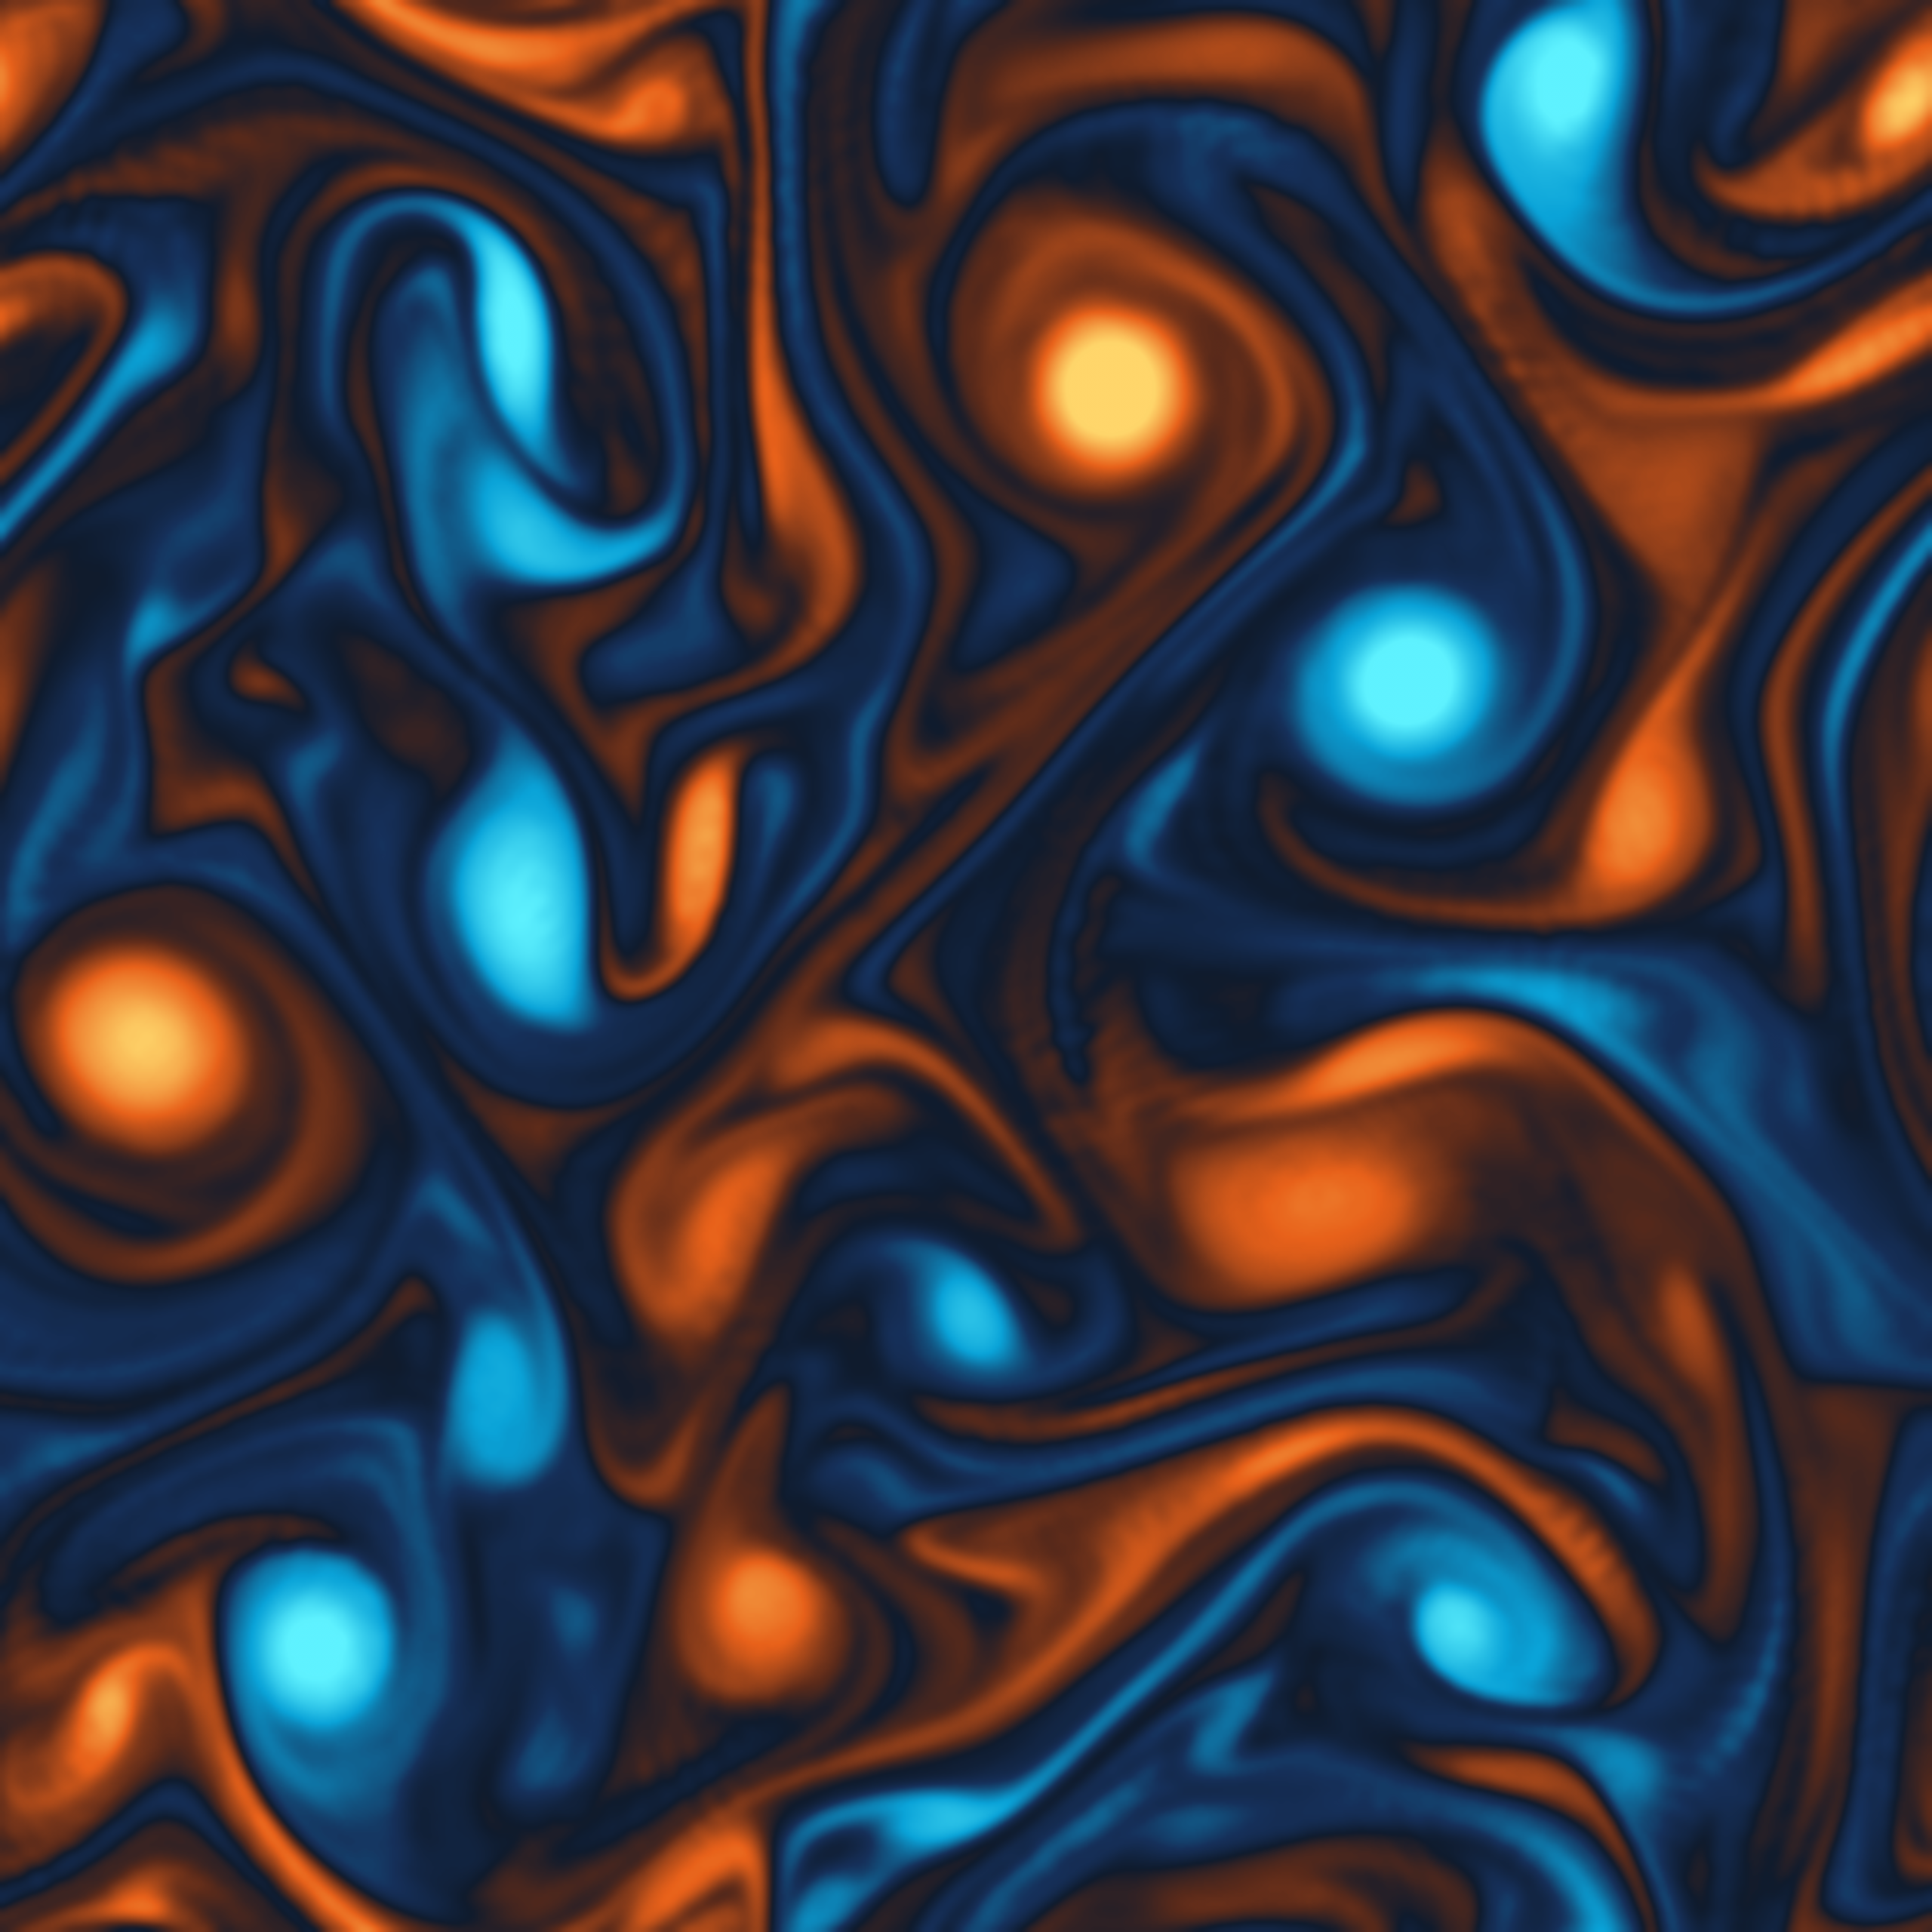
\includegraphics[width=7.125in]{art_ns.png}};
\end{scope}
% front text
\node[text=ivory,align=center] at (\FrontC,9.26) {\fontsize{42}{48}\selectfont\scshape On Hilbert's};
\node[text=ivory,align=center] at (\FrontC,8.49) {\fontsize{42}{48}\selectfont\scshape 6th Problem};
\draw[gold,line width=0.6pt] (\FrontC-1.33,7.90) -- (\FrontC+1.33,7.90);
\node[text=gold,align=center] at (\FrontC,7.45) {\fontsize{16.5}{21}\selectfont\itshape Probability, Mechanics and Bayesian Computation};
\node[text=ivory,align=center] at (\FrontC,6.93) {\fontsize{17.5}{22}\selectfont\scshape Nick Polson \quad\textperiodcentered\quad Vadim Sokolov};
% spine
\node[text=ivory,rotate=-90,anchor=center] at (\SpineC,6.21) {\fontsize{14}{16}\selectfont\scshape On Hilbert's 6th Problem};
\node[text=gold,rotate=-90,anchor=center] at (\SpineC,1.76) {\fontsize{11}{13}\selectfont\scshape Polson \,\textperiodcentered\, Sokolov};
% back cover blurb
\node[text=ivory,anchor=north west,text width=5.6in,align=justify] at (0.75,9.36) {%
\fontsize{11.25}{15.2}\selectfont
{\fontsize{16.5}{21}\selectfont\scshape\color{gold} From atoms to continua, and back\par}
\vspace{0.9em}
In 1900 David Hilbert asked for a mathematical treatment of the axioms of physics, beginning with probability and mechanics, and for the limiting processes that lead from the atomistic view to the laws of motion of continua. A century and a quarter later Kolmogorov's axioms have settled the first half, and the passage from hard spheres to the Boltzmann equation and on to the Navier Stokes equations has been carried out for long times.\par
\vspace{0.6em}
This book tells that story and adds a second half: the inverse passage, from observed fluids back to the states that produced them. Henri Poincar\'e, who examined Bachelier's thesis in the year of Hilbert's address, is a central figure, from recurrence and the method of arbitrary functions to the quanta and the conjecture that Perelman settled with an entropy from statistical mechanics.\par
\vspace{0.6em}
Topics include de Finetti and Sanov, Brownian motion and Yor's identities read as algorithms, Thorin measures and shot noise, Perelman's entropy and the uncertainty principle, Nelson's stochastic mechanics, Lanford's theorem and Kac's program, hydrodynamic limits, Bayesian inference on the Navier Stokes solution manifold with adjoint sufficient statistics and learned posterior generators, blowup and turbulence, Lee Yang zeros, Schr\"odinger bridges and generative Bayesian computation, filters and gates, and the thermodynamics of information. A final chapter builds a bridge to Hilbert's eighth problem through the de Bruijn Newman heat flow. A chapter on ergodic theory, a chapter on the method of types and moment conditioning, and a section on Lanford windows complete the foundations; every chapter closes with exercises, and computed figures illustrate the book throughout.\par
\vspace{0.9em}
{\itshape Nick Polson is Professor of Econometrics and Statistics at the Booth School of Business, University of Chicago. Vadim Sokolov is Associate Professor at George Mason University.}\par
};
% barcode area kept clear (KDP places barcode here)
\fill[white] (4.875,0.375) rectangle (6.875,1.575);
\end{tikzpicture}
\end{document}
"   (twice),
% then check: kdp.py cover <interior.pdf> --cover cover.pdf. Without the definition the count below is used.
\providecommand\InteriorPages{548}
\documentclass{article}
\usepackage{tikz,graphicx,xcolor}
\pgfmathsetmacro\Spine{\InteriorPages*0.002252}
\pgfmathsetmacro\W{14.25+\Spine}
\pgfmathsetmacro\FrontL{7.125+\Spine}
\pgfmathsetmacro\FrontC{\FrontL+3.5}
\pgfmathsetmacro\SpineC{7.125+\Spine/2}
\usepackage[paperwidth=\W in,paperheight=10.25in,margin=0in]{geometry}
\usepackage[T1]{fontenc}
\usepackage[sc]{mathpazo}
\usepackage[none]{hyphenat}
\definecolor{navy}{HTML}{0F1B2D}
\definecolor{gold}{HTML}{D9B86C}
\definecolor{ivory}{HTML}{EFE6D2}
\pagestyle{empty}
\begin{document}
\noindent\begin{tikzpicture}[x=1in,y=1in,remember picture,overlay,shift={(current page.south west)}]
% background
\fill[navy] (0,0) rectangle (\W,10.25);
% front artwork, bleeding off right and bottom, cropped at the top below the authors
\begin{scope}
\clip (\FrontL,0) rectangle (\W,6.6);
\node[anchor=south west,inner sep=0] at (\FrontL,0) {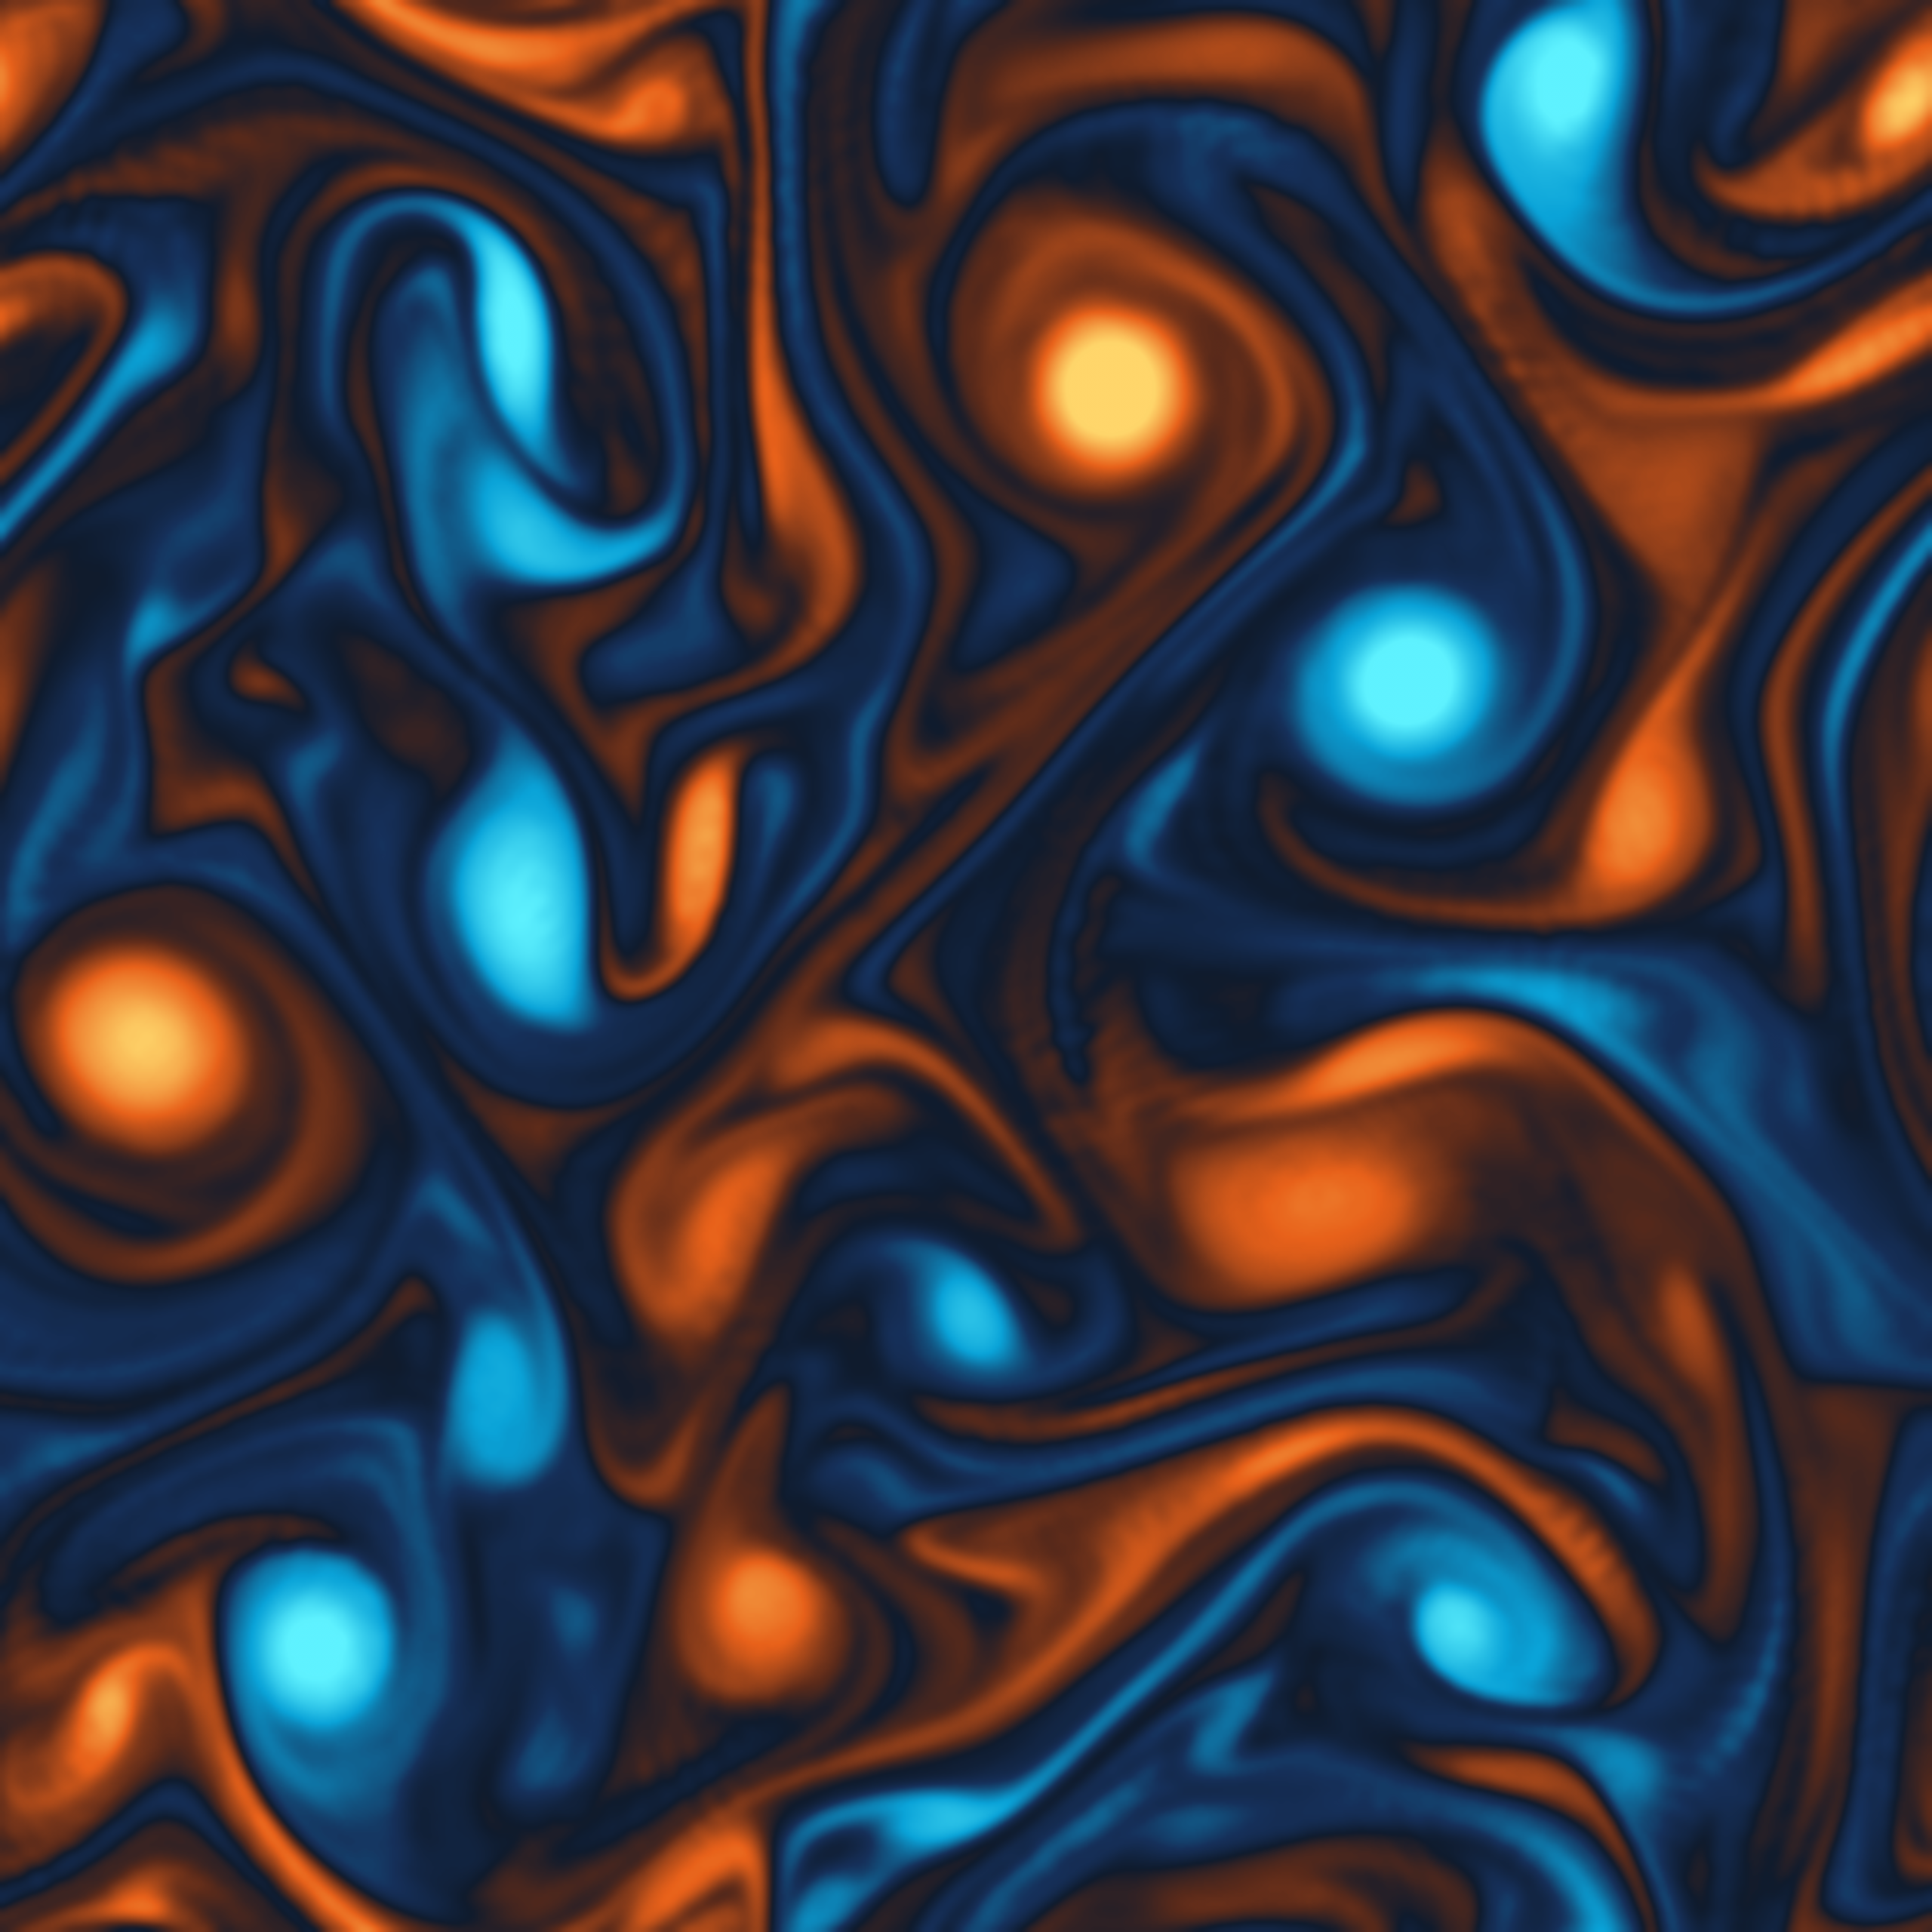
\includegraphics[width=7.125in]{art_ns.png}};
\end{scope}
% front text
\node[text=ivory,align=center] at (\FrontC,9.26) {\fontsize{42}{48}\selectfont\scshape On Hilbert's};
\node[text=ivory,align=center] at (\FrontC,8.49) {\fontsize{42}{48}\selectfont\scshape 6th Problem};
\draw[gold,line width=0.6pt] (\FrontC-1.33,7.90) -- (\FrontC+1.33,7.90);
\node[text=gold,align=center] at (\FrontC,7.45) {\fontsize{16.5}{21}\selectfont\itshape Probability, Mechanics and Bayesian Computation};
\node[text=ivory,align=center] at (\FrontC,6.93) {\fontsize{17.5}{22}\selectfont\scshape Nick Polson \quad\textperiodcentered\quad Vadim Sokolov};
% spine
\node[text=ivory,rotate=-90,anchor=center] at (\SpineC,6.21) {\fontsize{14}{16}\selectfont\scshape On Hilbert's 6th Problem};
\node[text=gold,rotate=-90,anchor=center] at (\SpineC,1.76) {\fontsize{11}{13}\selectfont\scshape Polson \,\textperiodcentered\, Sokolov};
% back cover blurb
\node[text=ivory,anchor=north west,text width=5.6in,align=justify] at (0.75,9.36) {%
\fontsize{11.25}{15.2}\selectfont
{\fontsize{16.5}{21}\selectfont\scshape\color{gold} From atoms to continua, and back\par}
\vspace{0.9em}
In 1900 David Hilbert asked for a mathematical treatment of the axioms of physics, beginning with probability and mechanics, and for the limiting processes that lead from the atomistic view to the laws of motion of continua. A century and a quarter later Kolmogorov's axioms have settled the first half, and the passage from hard spheres to the Boltzmann equation and on to the Navier Stokes equations has been carried out for long times.\par
\vspace{0.6em}
This book tells that story and adds a second half: the inverse passage, from observed fluids back to the states that produced them. Henri Poincar\'e, who examined Bachelier's thesis in the year of Hilbert's address, is a central figure, from recurrence and the method of arbitrary functions to the quanta and the conjecture that Perelman settled with an entropy from statistical mechanics.\par
\vspace{0.6em}
Topics include de Finetti and Sanov, Brownian motion and Yor's identities read as algorithms, Thorin measures and shot noise, Perelman's entropy and the uncertainty principle, Nelson's stochastic mechanics, Lanford's theorem and Kac's program, hydrodynamic limits, Bayesian inference on the Navier Stokes solution manifold with adjoint sufficient statistics and learned posterior generators, blowup and turbulence, Lee Yang zeros, Schr\"odinger bridges and generative Bayesian computation, filters and gates, and the thermodynamics of information. A final chapter builds a bridge to Hilbert's eighth problem through the de Bruijn Newman heat flow. A chapter on ergodic theory, a chapter on the method of types and moment conditioning, and a section on Lanford windows complete the foundations; every chapter closes with exercises, and computed figures illustrate the book throughout.\par
\vspace{0.9em}
{\itshape Nick Polson is Professor of Econometrics and Statistics at the Booth School of Business, University of Chicago. Vadim Sokolov is Associate Professor at George Mason University.}\par
};
% barcode area kept clear (KDP places barcode here)
\fill[white] (4.875,0.375) rectangle (6.875,1.575);
\end{tikzpicture}
\end{document}
"   (twice),
% then check: kdp.py cover <interior.pdf> --cover cover.pdf. Without the definition the count below is used.
\providecommand\InteriorPages{548}
\documentclass{article}
\usepackage{tikz,graphicx,xcolor}
\pgfmathsetmacro\Spine{\InteriorPages*0.002252}
\pgfmathsetmacro\W{14.25+\Spine}
\pgfmathsetmacro\FrontL{7.125+\Spine}
\pgfmathsetmacro\FrontC{\FrontL+3.5}
\pgfmathsetmacro\SpineC{7.125+\Spine/2}
\usepackage[paperwidth=\W in,paperheight=10.25in,margin=0in]{geometry}
\usepackage[T1]{fontenc}
\usepackage[sc]{mathpazo}
\usepackage[none]{hyphenat}
\definecolor{navy}{HTML}{0F1B2D}
\definecolor{gold}{HTML}{D9B86C}
\definecolor{ivory}{HTML}{EFE6D2}
\pagestyle{empty}
\begin{document}
\noindent\begin{tikzpicture}[x=1in,y=1in,remember picture,overlay,shift={(current page.south west)}]
% background
\fill[navy] (0,0) rectangle (\W,10.25);
% front artwork, bleeding off right and bottom, cropped at the top below the authors
\begin{scope}
\clip (\FrontL,0) rectangle (\W,6.6);
\node[anchor=south west,inner sep=0] at (\FrontL,0) {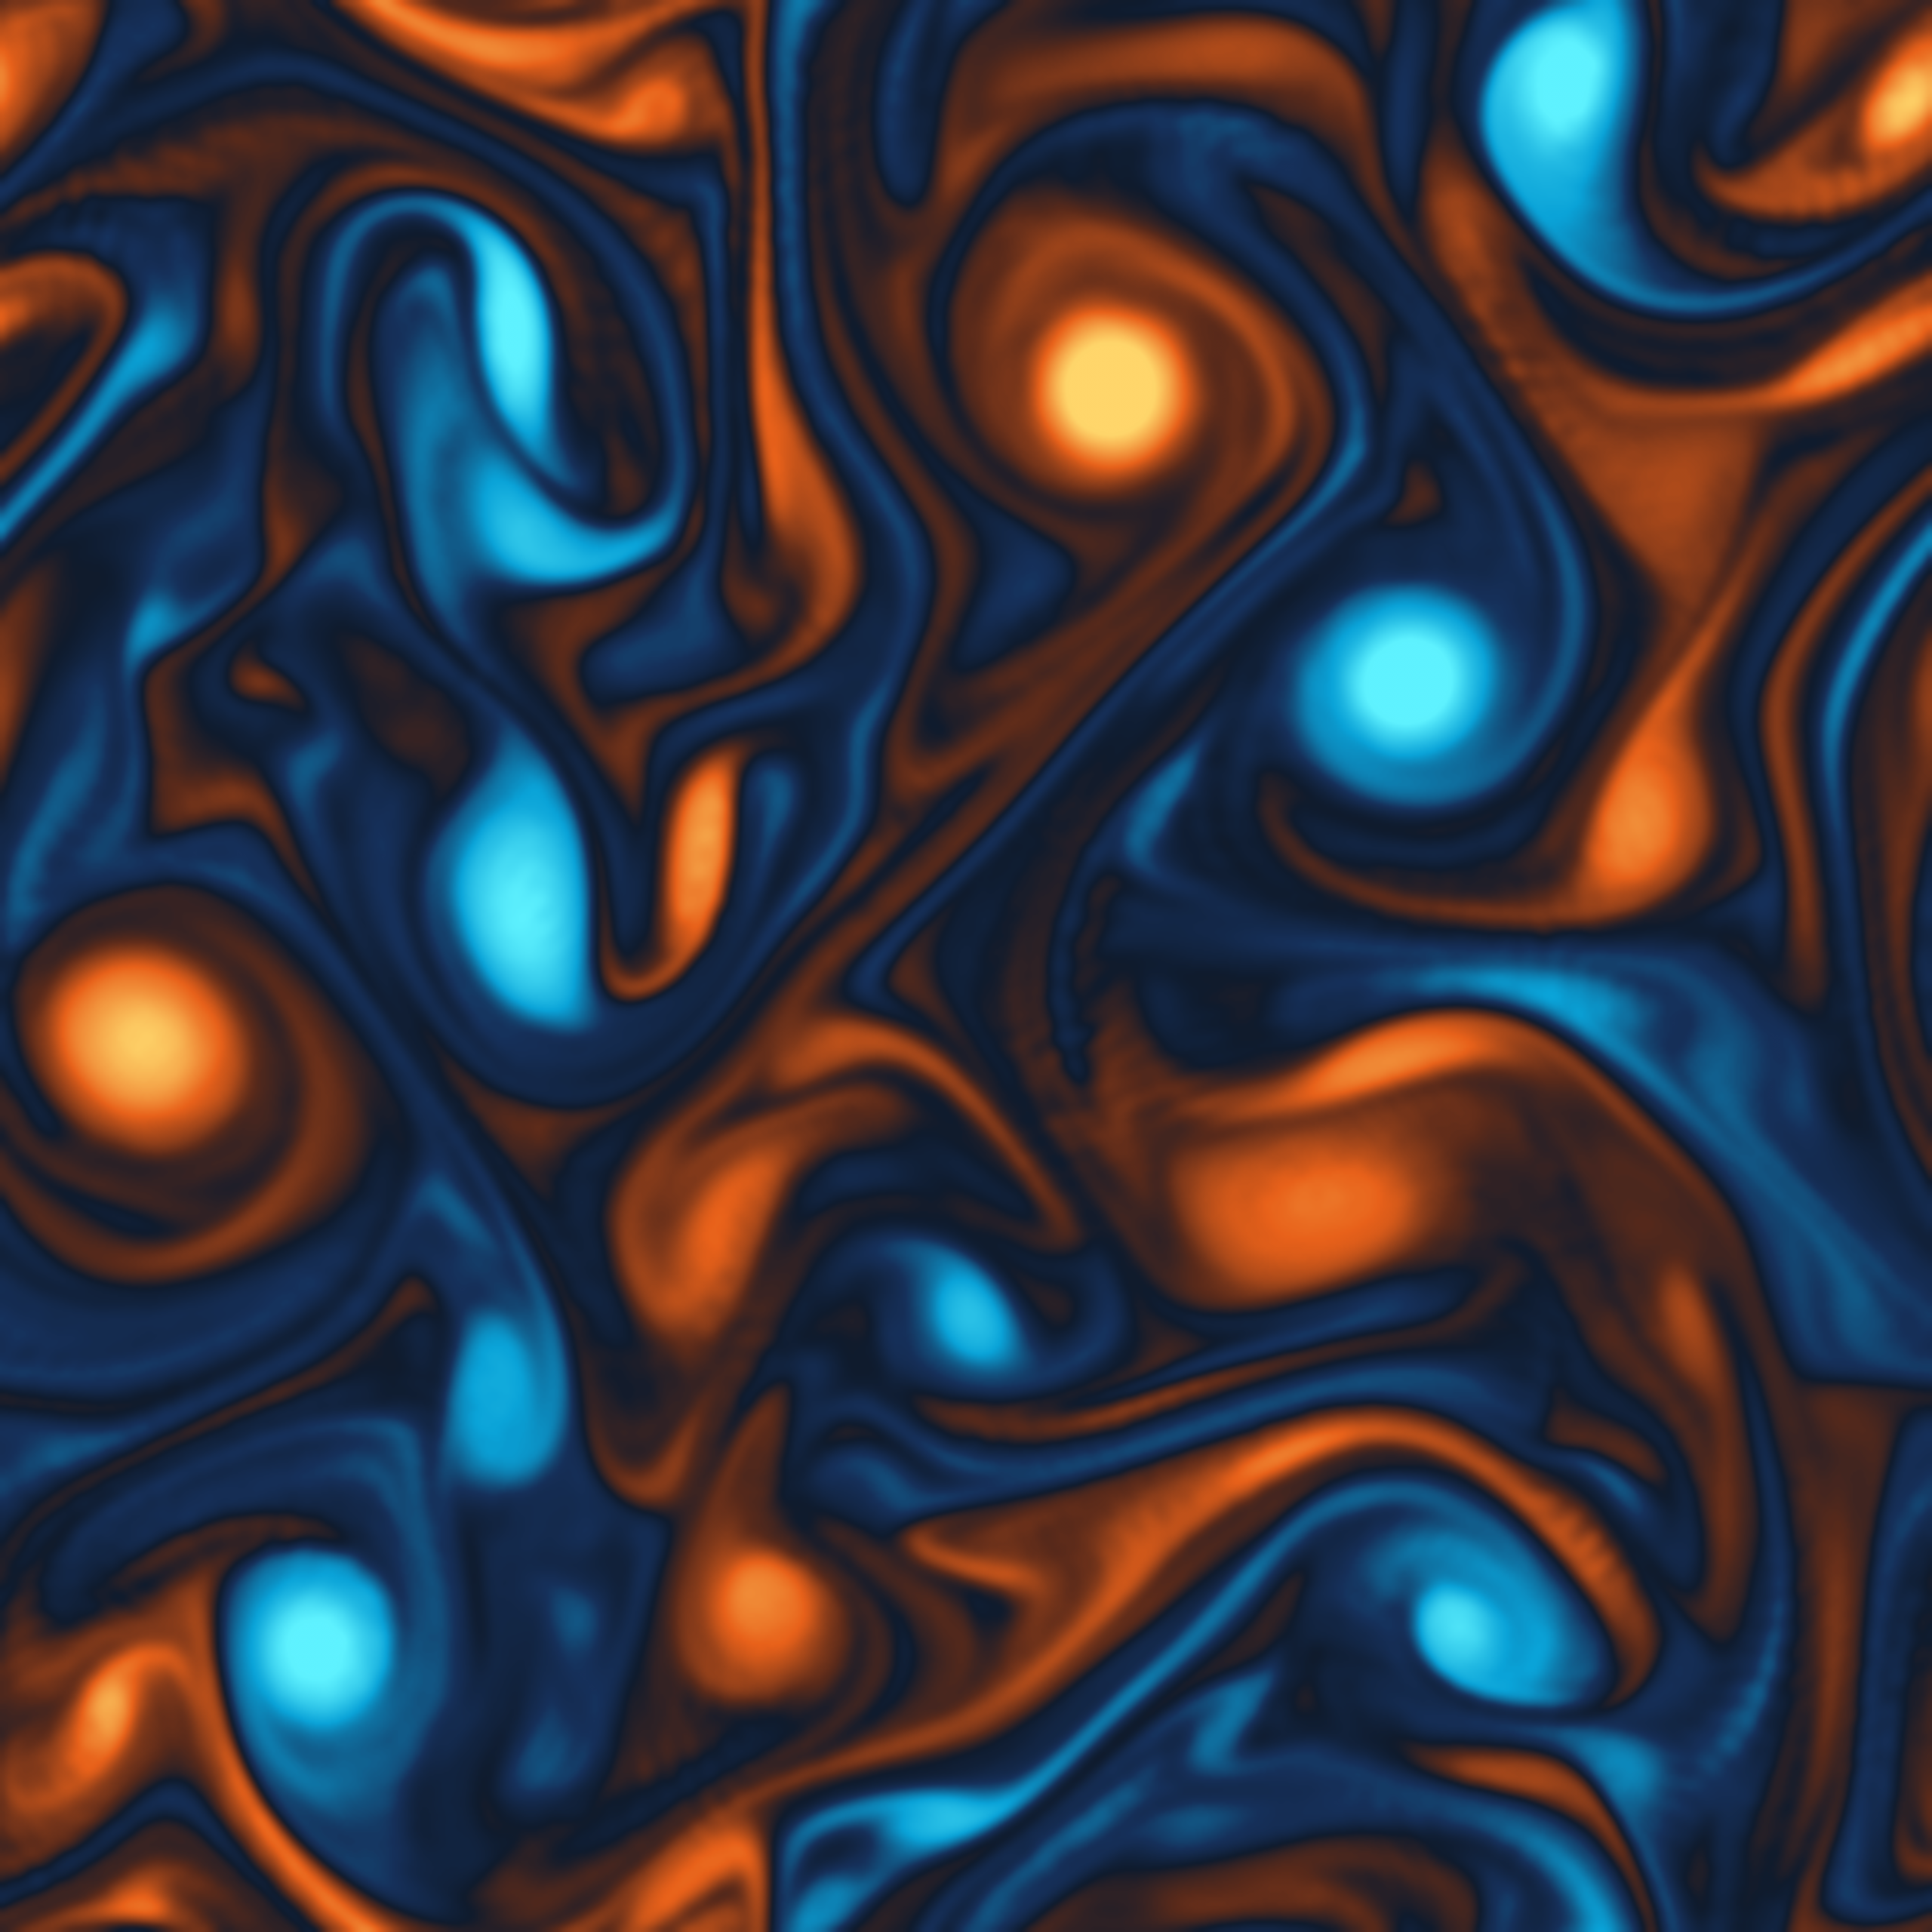
\includegraphics[width=7.125in]{art_ns.png}};
\end{scope}
% front text
\node[text=ivory,align=center] at (\FrontC,9.26) {\fontsize{42}{48}\selectfont\scshape On Hilbert's};
\node[text=ivory,align=center] at (\FrontC,8.49) {\fontsize{42}{48}\selectfont\scshape 6th Problem};
\draw[gold,line width=0.6pt] (\FrontC-1.33,7.90) -- (\FrontC+1.33,7.90);
\node[text=gold,align=center] at (\FrontC,7.45) {\fontsize{16.5}{21}\selectfont\itshape Probability, Mechanics and Bayesian Computation};
\node[text=ivory,align=center] at (\FrontC,6.93) {\fontsize{17.5}{22}\selectfont\scshape Nick Polson \quad\textperiodcentered\quad Vadim Sokolov};
% spine
\node[text=ivory,rotate=-90,anchor=center] at (\SpineC,6.21) {\fontsize{14}{16}\selectfont\scshape On Hilbert's 6th Problem};
\node[text=gold,rotate=-90,anchor=center] at (\SpineC,1.76) {\fontsize{11}{13}\selectfont\scshape Polson \,\textperiodcentered\, Sokolov};
% back cover blurb
\node[text=ivory,anchor=north west,text width=5.6in,align=justify] at (0.75,9.36) {%
\fontsize{11.25}{15.2}\selectfont
{\fontsize{16.5}{21}\selectfont\scshape\color{gold} From atoms to continua, and back\par}
\vspace{0.9em}
In 1900 David Hilbert asked for a mathematical treatment of the axioms of physics, beginning with probability and mechanics, and for the limiting processes that lead from the atomistic view to the laws of motion of continua. A century and a quarter later Kolmogorov's axioms have settled the first half, and the passage from hard spheres to the Boltzmann equation and on to the Navier Stokes equations has been carried out for long times.\par
\vspace{0.6em}
This book tells that story and adds a second half: the inverse passage, from observed fluids back to the states that produced them. Henri Poincar\'e, who examined Bachelier's thesis in the year of Hilbert's address, is a central figure, from recurrence and the method of arbitrary functions to the quanta and the conjecture that Perelman settled with an entropy from statistical mechanics.\par
\vspace{0.6em}
Topics include de Finetti and Sanov, Brownian motion and Yor's identities read as algorithms, Thorin measures and shot noise, Perelman's entropy and the uncertainty principle, Nelson's stochastic mechanics, Lanford's theorem and Kac's program, hydrodynamic limits, Bayesian inference on the Navier Stokes solution manifold with adjoint sufficient statistics and learned posterior generators, blowup and turbulence, Lee Yang zeros, Schr\"odinger bridges and generative Bayesian computation, filters and gates, and the thermodynamics of information. A final chapter builds a bridge to Hilbert's eighth problem through the de Bruijn Newman heat flow. A chapter on ergodic theory, a chapter on the method of types and moment conditioning, and a section on Lanford windows complete the foundations; every chapter closes with exercises, and computed figures illustrate the book throughout.\par
\vspace{0.9em}
{\itshape Nick Polson is Professor of Econometrics and Statistics at the Booth School of Business, University of Chicago. Vadim Sokolov is Associate Professor at George Mason University.}\par
};
% barcode area kept clear (KDP places barcode here)
\fill[white] (4.875,0.375) rectangle (6.875,1.575);
\end{tikzpicture}
\end{document}
